\documentclass[10pt,a4paper]{article}
\usepackage[T1]{fontenc}
\usepackage[a4paper]{geometry}
\usepackage{xcolor}
\usepackage{amssymb}
\usepackage{amsmath}
\usepackage{graphicx}
\usepackage{tabularx}
\usepackage{multirow}
\usepackage{subfigure}
\usepackage{verbatim}
\usepackage{fancyhdr}
\usepackage{listings}
\usepackage{../common/espacs}

%\input{../common/commands.tex}


\title{Exercise Session 9}
\date{December 14, 2012}

\pagestyle{fancy}
\headheight 35pt

\newcommand{\vv}[1]{\mathbf{#1}}

\begin{document}
\lstset{language=[ISO]C++}
\maketitle

\section*{Esercizio 1}

Starting from the example \texttt{QuadratureRule/baseVersion}
\begin{enumerate}
  \item extend the use of GetPot in order to pass the integrand function
  directly from the data file

  \item add a Gaussian quadrature rule, templatized on the number of quadrature
  points. The Gaussian rule should derive from the common base class
  \cpp{StandardQuadratureRule}. The points and weights can be computed using the
  \texttt{legendre\_rule} library

  \item compute the integral of the function
    \begin{align*}
    f(x) = e^x x
    \end{align*}
  in $[0,1]$ using all the available quadrature rules.

  \item implement a MonteCarlo quadrature rule, that also derives from
  \cpp{QuadratureRule}.
\end{enumerate}


%\subsection*{Exercise 1 solution}

The solution for the exercise is as follows
%
\lstset{basicstyle=\scriptsize\sf}
    \lstinputlisting{./src/all_in_one/bn-allinone.cpp}
\lstset{basicstyle=\sf}

First of all, we have defined a user type called \cpp{real}. If we want to
change the precision for the calculations, it will be sufficient to just change
the definition for the \cpp{real} type. All the code would be updated
coherently.

In order to have the possibility to pass an arbitrary function to the method
that performs the evaluation of the zero we use a \emph{function pointer}. The
instruction
\begin{lstlisting}
typedef real (*fctptr)(real);
\end{lstlisting}
defines a type \cpp{fctptr} as a pointer to a function that have a \cpp{real} as
argument and thta have a \cpp{real} as return value.

we can adopt different strategies to stop the iterations of a method that
computes a zero. When the function derivative absolute value is close to $1$ in
the neighborhood of the zero an efficient way to set a stop criterion is by
using the \emph{residual}. More specifically, we consider that the method as
converged at the iteration $k$ when $\module{\function{f}{x\iter{k}}} <
\cpp{tol}$.

An alternative way, based on a check on the \emph{increment}, is instead
suitable for fixed point iterations when the derivative of the iteration
function $\function{\phi}{\cdot}$ is far away from $1$ in modulus near the zero.
The criterion stops the iterations when $\module{x\iter{k+1} - x\iter{k}} <
\cpp{tol}$. For the Newton's method, where $\function{\phi'}{\alpha} = 0$ by
definition, the check on the increment is a typical choice. The implementation
takes care of the different types of stop criteria with an \emph{enumeration},
called \cpp{checkT}. Every method has a member \cpp{M\_check} of type
\cpp{checkT} that chooses the convergence criterion.

If we compile with
\begin{verbatim}
    g++ -o bn-allinone bn-allinone.cpp -Wall
\end{verbatim}
and execute the resulting program we get
\begin{verbatim}
0.707107        27
0.707107        7
0.707107        14 1
\end{verbatim}



\section*{Es. 2}

Keeping in mind the first exercise

\begin{enumerate}

    \item separate the program in multiple files, in a modular way, so that
    code usability is improved. Hint: group all implementations in a source
    file, add a correspondent header file and keep the main in a third file.

    \item repeat the last point of the first exercise.

    \item knowing that the exact solution for the previous point is
    $x=\sqrt{0.5}$, modify the code in order to save the distance between the
    current approximate solution and previous approximate solution in a file.
    Plot the solution with \texttt{gnuplot}. Comment the results using the
    theory.

\end{enumerate}

%\subsection*{Exercise 2 solution}

Here follows the listing for the \emph{header file} that contains all the
declarations of the functions in the code.
% zerofun.hpp
\lstset{basicstyle=\scriptsize\sf}
    \lstinputlisting[caption=Function declarations for computing the zero of a
    function.] {src/zerofun.hpp}
\lstset{basicstyle=\sf}

We put the corresponding definitions in the \emph{source file}
\texttt{zerofun.cpp}:
\lstset{basicstyle=\scriptsize\sf}
    \lstinputlisting[caption=Function definitions for computing the zero of a
    function.] {src/zerofun.cpp}
\lstset{basicstyle=\sf}

The instruction \texttt{assert(u*f(b)<0.0);} is used to perform a simple error
checking. If the boolean instruction inside is not verified, the program stop
immediately and an error message is generated.

We have also the listing for the file \texttt{bn.cpp} that contains the main
program
\lstset{basicstyle=\scriptsize\sf}
    \lstinputlisting[caption=function definition and main program.]
    {src/bn.cpp}
\lstset{basicstyle=\sf}

The compilation can be peformed with
\begin{verbatim}
g++  -c -o bn.o bn.cpp -Wall
g++  -c -o zerofun.o zerofun.cpp -Wall
g++  -o bn bn.o zerofun.o
\end{verbatim}

The files \texttt{bn.o} and \texttt{zerofun.o} are the translation to object
code of the type and function definitions that we wrote in the corresponding
source files. The executable \texttt{bn} is created throught the \emph{linking}
of the object files together with the necessary libraries.

The \cpp{assert} can be disabled with the \cpp{-DNDEBUG} flag that must be
passed to the compiler when compiling files that contain it, i.e.
\begin{verbatim}
g++  -c -o bn.o bn.cpp -Wall
g++  -c -o zerofun.o zerofun.cpp -Wall -DNDEBUG
g++  -o bn bn.o zerofun.o
\end{verbatim}

In order to graphically see the error, it is possible to pass two additional
arguments to the functions  \texttt{bisection}, \texttt{newton} and
\texttt{robust}. The first one is the exact solution, while the second is the
name of the file for the output.
The listing for the \texttt{bng.cpp} file is as follows
\lstset{basicstyle=\scriptsize\sf}
    \lstinputlisting[caption=Function definition and main program.]
        {src/withGnuplot/bng.cpp}
\lstset{basicstyle=\sf}

we note at the end the call to the operating system that uses the file
\texttt{print\_data} with the following commands
\begin{verbatim}
set terminal png
set output "graph.png"
plot "data" with lines
\end{verbatim}
The listing for \texttt{zerofung.hpp} is basically the same as
\texttt{zerofun.hpp}, while the listing for \texttt{zerofung.cpp} is
\lstset{basicstyle=\scriptsize\sf}
    \lstinputlisting[caption=Definitions for the functions to compute a zero of
        a function.]{src/withGnuplot/zerofung.cpp}
\lstset{basicstyle=\sf}

Note how the functions \texttt{bisection} and \texttt{newton} manage the file.
First of all it is declared, using the scope resolution operator \cpp{::} to
access the members in the \cpp{std} namespace. Afterwards it is opened in the
out mode for \texttt{bisection}, and out and app for \texttt{newton}.i This
means that in the second case the files are written at the end of the file,
without deleting any previous content. There is also a test to verify that the
file has been properly opened. The data output is performed inside the loops in
a way that is totally similar to printing to screen. at the end of each function
the file is closed.

This is the graph generated by the code
\begin{figure}[!h]
    \centering
    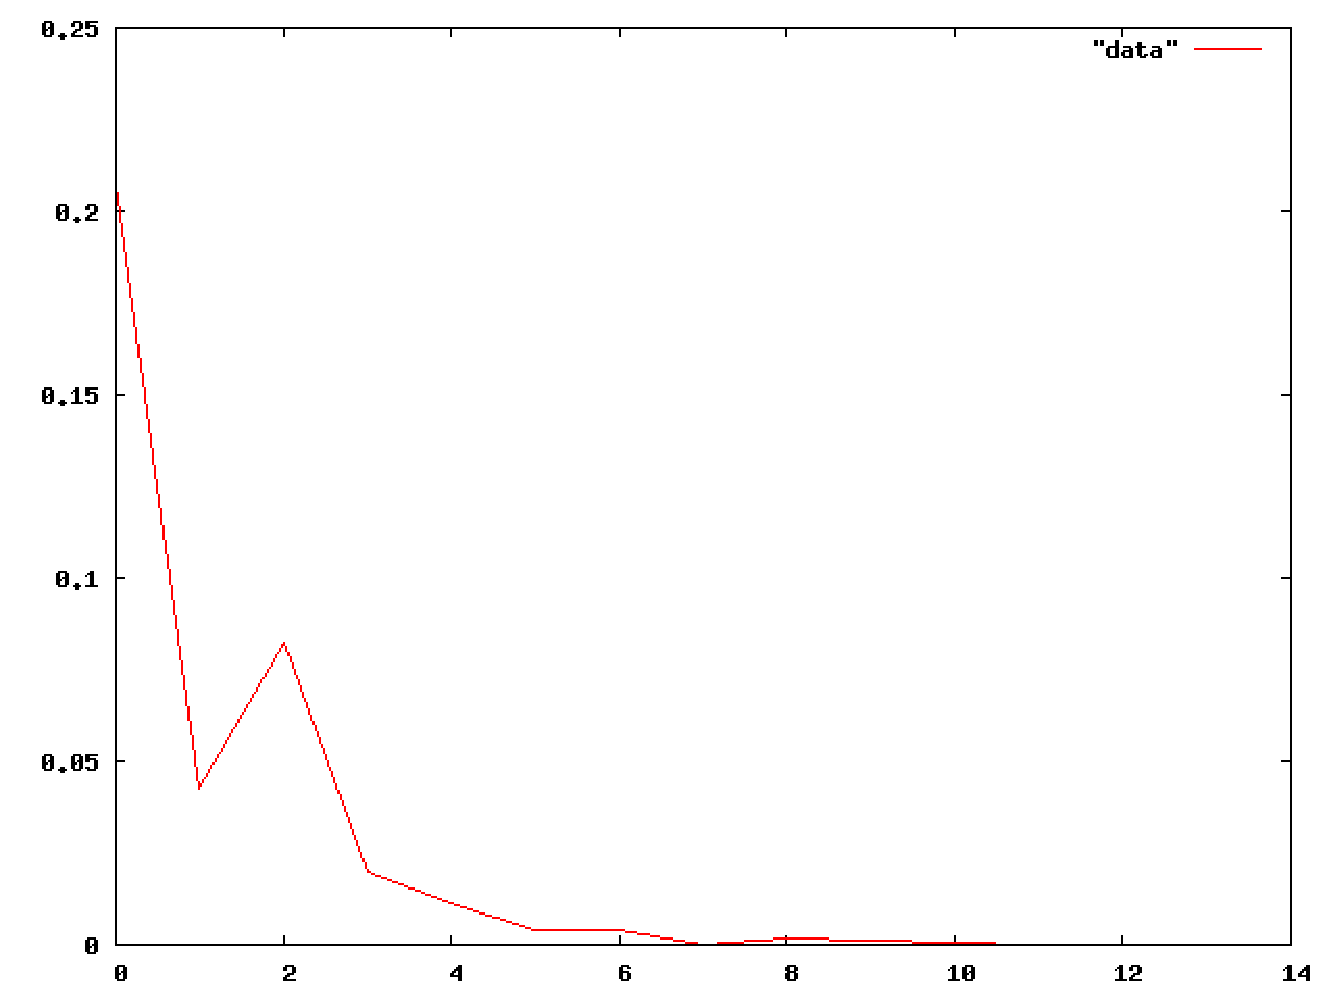
\includegraphics[width=0.7\textwidth]{./images/graph}
\end{figure}


\end{document}
